\chapter{应用设计与实现}
\label{cha:experiment}

\section{应用功能设计}
\label{sec:app_design}
第一步,我们需要对复杂的开发过程进行组织,设计一个产品线系统\cite{Yang},它是CMU/SEI提出的产品开发组织方式,集中体现了软件复用思想。当我们按照需求设计好功能之后,才能对应用整体有一个更好的把控,开发起来也会更加顺畅。
\begin{figure}[h]
	\centering
	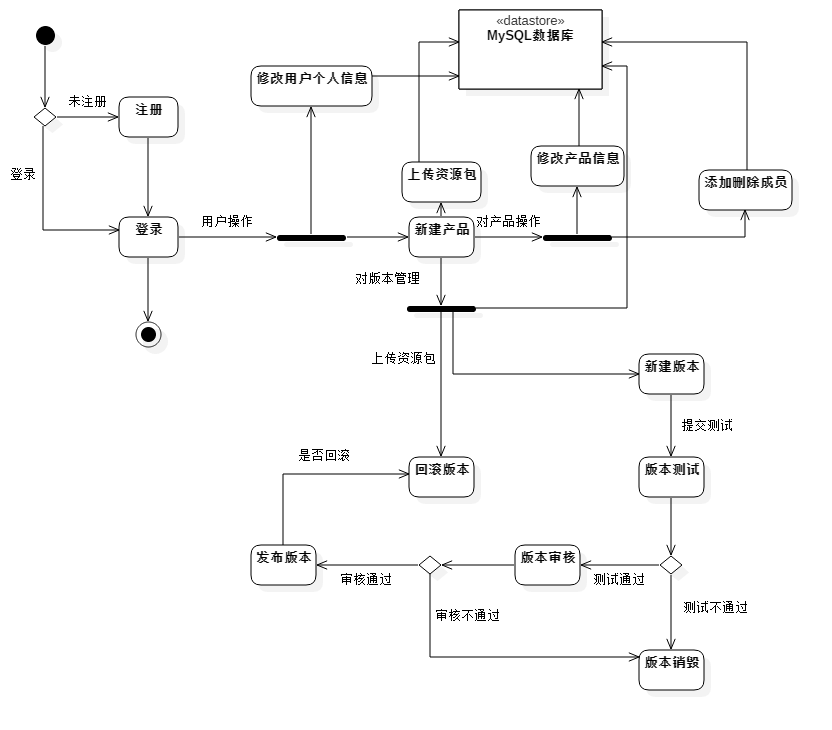
\includegraphics[width=0.8\textwidth]{image/UML/ActivityDiagram.png}
	\caption{应用功能设计}
	\label{fig:app}
\end{figure}
从上面的活动图可以看出,活动流程包含了三个方面:账户管理、产品管理(包括产品信息的修改和成员的增删)、对产品版本的管理
\begin{itemize}
	\item 账户管理的功能包括登录,注册,注销,更改个人信息,基本满足了对于应用使用者的需求
	\item 产品管理的功能包括修改产品信息,添加某角色(产品开发者/测试员)的成员,删除某角色的成员,更换管理员,新建产品(即提交新产品的信息和新建产品的第一个版本)
	\item 版本管理的功能包括新建版本(需要上传新版本的资源包),版本流程的管理(测试,审核,发布),版本回滚
	\begin{figure}[h]
		\centering
		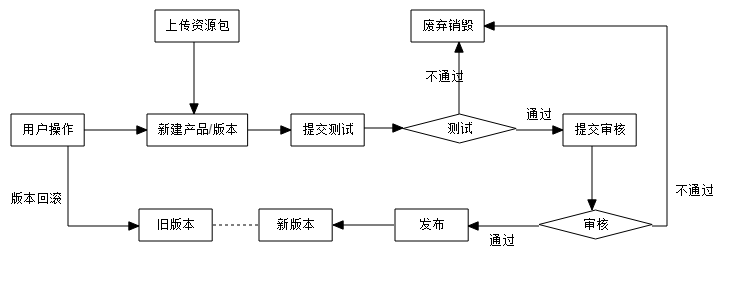
\includegraphics[width=0.8\textwidth]{image/UML/FlowchartDiagram.png}
		\caption{版本管理流程}
		\label{fig:version}
	\end{figure}
	\item 最后还有成员管理,这个功能其实包括在产品管理里面,这里主要说明一下成员和用户的区别。

	两者之间的区别在于,一个用户可以是多个成员,甚至是多个不同产品的相同或者不同的成员,而每个产品下都有三种成员:产品管理者,产品开发者,产品测试员,他们拥有不同的权限。所以成员其实跟用户和产品都有关系,是联系两个模型的重要枢纽
\end{itemize}

\section{前端架构}
\label{sec:Front-end_architecture}
\begin{figure}[h]
	\centering
	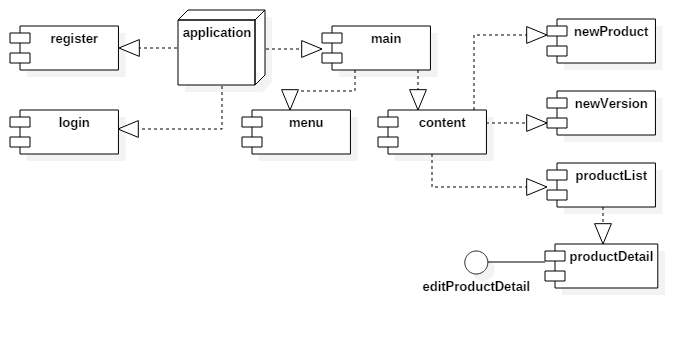
\includegraphics[width=0.8\textwidth]{image/UML/ComponentDiagram.png}
	\caption{前端架构}
	\label{fig:frame}
\end{figure}
angular的优点是模块化和组件化,将每个页面封装成一个个组件,利用路由功能在不同的组件之间跳跃,实现页面的快速跳转。
同时,利用模板语法和数据绑定,使得前后端开发分离,我们只需要从后台获得关键数据,即可在前台的HTML模板中填入数据,渲染页面。与传统web系统相区别,web应用能为用户提供丰富的操作,能够随用户操作不断更新视图而不进行url跳转。ng官方也声明它更适用于开发CRUD应用,即数据操作比较多的应用,而非是游戏或图像处理类应用。为了实现这些,ng引入了一些非常棒的特性,包括模板机制、数据绑定、模块、指令、依赖注入、路由。通过数据与模板的绑定,能够让我们摆脱繁琐的DOM操作,而将注意力集中在业务逻辑上。

所以第二步,我们要做的是将应用的功能分成多个模块,将框架分成多个层级:1. 将整体的功能分成7个模块,分别实现登录,注册,显示菜单,显示产品列表,新建产品,新建版本,接收系统信息等。2.将这些功能整合到一起,分成四个层级,登录,注册,主要界面是第一层;主要界面包括,显示菜单,显示内容,这是第二层;显示内容将整合剩余模块的展示,产品列表,新建产品页面,新建版本页面,接收系统信息页面都将在这里显示,这是第三层;而显示产品列表通常是不能满足需求的,列表里面的每个产品都应该能导向一个显示详情的页面,而这个就是第四层。

因此,上图的组件架构可以表示为:
\begin{itemize}
	\item login
	\item register
	\item main
	\begin{itemize}
		\item menu
		\item content
			\begin{itemize}
				\item newProduct
				\item newVersion
				\item productList
				\begin{itemize}
					\item productDetail
				\end{itemize}
			\end{itemize}
	\end{itemize}
\end{itemize}
\section{界面设计}
\label{sec:UI}
第三步是要敲定整个应用的UI风格,以及大致有什么功能组件,应该如何排版,这样可以从头到尾梳理一遍所有的功能,不至于在开发过程中手忙脚乱。阿里的ant design\cite{Zorro}针对angular封装了对应的UI风格和许多实用的组件供开发者使用,这个框架叫做ng-Zorro,它能让开发者不必花费过多的时间在UI的设计上面,让开发的周期变得更短。当然,这并不意味着界面方面就可以轻松完成,如何将框架和项目更好地组合起来,如何利用在框架的规范下实现你的逻辑,如何利用这些工具来更好地实现你想要的东西,这才是最需要推敲的事情。例如,如何利用Zorro的栅格布局让应用编程一个响应式的网页应用;如何实现弹窗以及在两者之间传递事件和数据,如何使文件上传功能按照自己想要的方式改造;选择什么样的组件才能让这个功能更具表现力等等。
		
使用方法:npm install ng-zorro-antd
\begin{itemize}
	\item 本应用的主要界面包括顶部功能栏,左侧边导航栏,以及剩下的内容展示区
	\item 顶部栏包括搜索输入框,查看系统邮件的入口,新建产品功能按钮,登出按钮
	\item 左侧导航栏显示了当前登陆用户的信息,以及该用户参与的项目导航列表
	\item 内容展示区则是界面中剩下的部分,不管是产品列表还是产品成员的展示,或者是新建版本、新建产品的显示都在这块区域
	\item 其余界面包括登录、注册界面,两个界面均填满整个浏览器窗口
\end{itemize}

\section{数据库设计}
\label{sec:database_design}
数据库是本应用不可或缺的重要部分,有了数据库,这个应用才有了灵魂。因此第四步,也是最关键的一步,是设计一个良好的数据库。这个数据库不但要存储整个应用所需要的所有数据,而且数据表之间还有较为紧密的联系,我们经常能碰到的情况是一个表不能将所有的数据都储存起来,比如有100个产品要储存名字和版本,每个产品有100个成员,每个成员要储存名字和手机号,对于关系型数据库来说,一个表是无法完美储存这些信息的,就算非要储存,也会多出很多冗余的数据,更别提体现出信息之间的相互关系了。但是,我们可以使用多个表来储存这些信息,如下图

\begin{figure}[h]
	\centering
	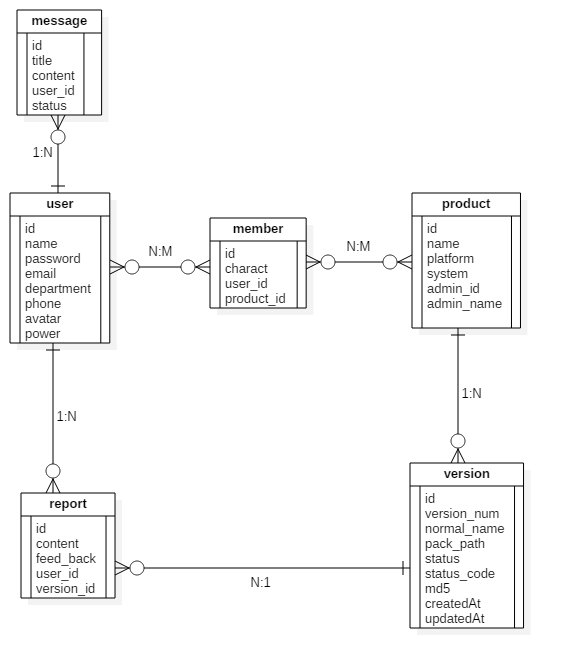
\includegraphics[width=0.8\textwidth]{image/UML/ERDDiagram.png}
	\caption{数据库设计}
	\label{fig:database}
\end{figure}
可以看到,本应用使用MySQL数据库建立一系列相互联系的表。之所以如此选择,一是因为本应用的各表之间的联系比较紧密,需要经常在多表之间进行联合查询,二是MySQL支持事务功能,对数据进行CRUD的时候能保持原子性。下面是数据库中各表的设计信息:
\begin{itemize}
	\item user表 
	
	\begin{figure}[h]
		\centering
		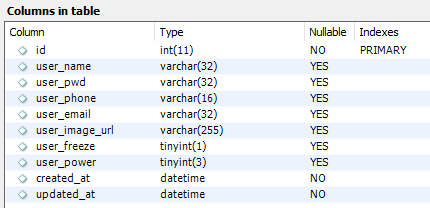
\includegraphics[width=0.8\textwidth]{image/database/users.png}
		\caption{数据库设计}
		\label{fig:u}
	\end{figure}
	用户表里面包含用户的个人信息,比如姓名,账号密码,手机号,邮箱等,储存着本应用的所有账户的信息
	\item product表 
		\begin{figure}[h]
		\centering
		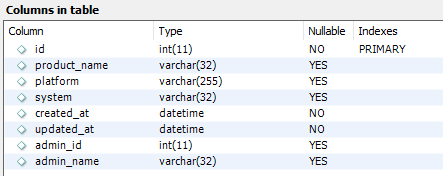
\includegraphics[width=0.8\textwidth]{image/database/product.png}
		\caption{数据库设计}
		\label{fig:p}
	\end{figure}
	产品表里面包含产品的所有信息,包括所属平台,操作系统,管理员等。
	而产品的版本信息由version表提供,我们将两个表建立1:N的关系,表示一个产品可以有多个版本,这样就可以通过join等MySQL操作获取到对应的version表的数据。
	产品的成员信息由member表提供,实际上,member表是表现出产品表和用户表之间的N:M关系的连接表,它将两个表的关系记录下来以方便查询,这样我们能很方便地将某个用户添加到某个产品的成员名下。
	\item member表 
		\begin{figure}[h]
		\centering
		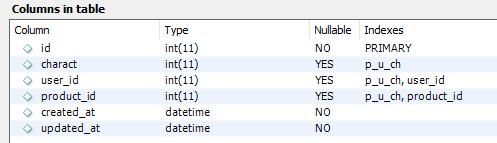
\includegraphics[width=0.8\textwidth]{image/database/member.png}
		\caption{数据库设计}
		\label{fig:database}
	\end{figure}
	如上面所说,该表是表现出产品表和用户表之间的N:M关系的连接表,因此它需要包括user和product两个表的外键user\_id和product\_id,同时,它也有自己的属性charact来表明这个成员是属于哪个权限的,是开发者还是测试员。
	\item version表 
	
		\begin{figure}[h]
		\centering
		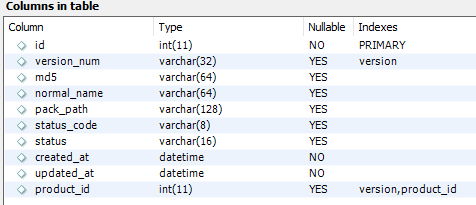
\includegraphics[width=0.8\textwidth]{image/database/versions.png}
		\caption{数据库设计}
		\label{fig:v}
	\end{figure}
	一个产品可以有多个版本,而version表记录着所有的版本,它包含版本号,当前状态,资源包的存储路径,文件的md5值,和product的外键product\_id。
	\item message表 
	
		\begin{figure}[h]
		\centering
		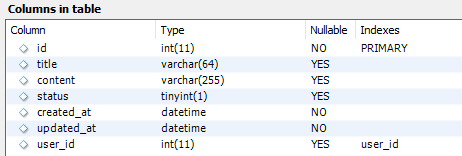
\includegraphics[width=0.8\textwidth]{image/database/message.png}
		\caption{数据库设计}
		\label{fig:m}
	\end{figure}
	这是存储向用户发送的系统提示邮件的数据表,记录着系统提示的title,content,接收人的id
	\item report表 
	
		\begin{figure}[h]
		\centering
		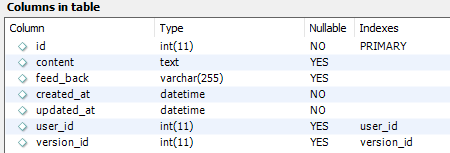
\includegraphics[width=0.8\textwidth]{image/database/report.png}
		\caption{数据库设计}
		\label{fig:r}
	\end{figure}
	这是向每个version的测试期提供的功能,每个测试员需要对该版本进行测试并填写测试报告,所以report表和version表其实是N:1的关系,每个version都有多个report。同时它还存储这提交人,提交日期,提交内容等数据,以给审核者提供参考,并可以保存审核员的批复意见。
\end{itemize}
由于前端数据尤其是离线数据可能因为很多的原因出现被更改甚至丢失的情况,因此在程序的设计过程中始终要牢记的一点就是保存在前端缓存中的数据是不可信的\cite{h5safe}。不能够根据其中的不可信数据做重要决策,并且将其不经验证直接保存在数据库之中\cite{safe}。
\section{后端开发}
\label{sec:Backend_development }
最后第五步,为应用提供一个服务器后台,所有前端的数据将由后台提供,后台将根据业务逻辑将数据进行整合操作,然后连接数据库进行操作。后端服务器采用express+nodejs进行搭建。用express可以快速搭建一个基于nodejs的服务器,我们只需要把精力都放在接口实现上即可。
将接口分门别类在对应的不同文件中,利用express的路由功能可以精确访问到接口。
而要使服务器能连接数据库,我们需要额外的模块,我们可以使用基于nodejs的mysql模块,
但是有一个热门的orm(Object Relationship Model)框架Sequelize\cite{Sequelize}对于描述表之间的关系,以及多表查询方面有更加好的解决方案,
同时Sequelize基于Promise实现异步流程控制,能更好地解决nodejs中数据库操作的回调地狱问题,
能够更方便我们对数据库进行操作,因此我们选用Sequelize来对数据库进行操作。
接下来对应用的三个主要方面的功能的后台流程实现进行简单介绍。
\subsection{用户管理}
\label{user_manage}
		账户的操作包括登录,注册,注销,更改个人信息,其工作流程如下:
		\begin{itemize}
			\item 用户注册
			
			注册页面,输入用户信息,包括用户名和密码,提交;
			后台检索数据库数据,是否存在同一个用户,不存在则创建此用户;
			返回用户信息,跳转到应用主页。
			\item 用户登录
			
			登录页面输入用户名和密码;
			后台检查用户名和密码是否正确;
			正确则返回信息并跳转到应用主页,而这个时候可以将比较常用的信息如用户名称,手机号等储存到本地储存中,这种存储方式是Html5提供的新的存储方式,区别于session和cookie,它可以永久储存数据,而且容量也比较大\cite{local}。
		\end{itemize}
			
\subsection{产品管理}
\label{product_manage}
		产品管理流程包括修改产品信息,修改(增删)产品成员
		\begin{itemize}
			\item 修改产品信息:
			提交新的产品信息到后台,由后台更新数据库,需要提供产品id作为产品的唯一凭证
			\item 获取产品的成员列表:
			在member表中按product\_id进行搜索,并根据不同的charact来区分不同的成员列表,将三个列表返回前台
			\item 添加成员:
			在用户列表中选择用户,提交用户id=A和产品id=B,并提交成员角色信息(产品开发者=2,产品测试员=3)
			后台在member表上添加一条数据,纪录提交的三个信息,这条成员信息表示的是A用户是B产品下的一个某角色的成员,如此就不需要在user和product表储存冗余的信息
			\item 删除成员:
			提交成员id,在member表上根据id删除对应的数据
			\item 新建产品:
			这个功能其实包括了新建第一个产品版本,只是多了需要提交产品的相关信息这个步骤,因此关于新建第一个版本的实现流程和新建任一版本的基本相同,在下一小节进行阐述
		\end{itemize}					
\subsection{版本管理}
\label{version_manage} 
		版本管理流程包括新建版本,版本从开发到发布的系列流程操控,版本回滚控制
		\begin{itemize}
			\item 文件上传功能:
			新建任何一个版本都避不过上传一个新的资源包的步骤,因此我们需要实现文件上传的功能,而version表上的每一条数据都与一个资源包相关。
			文件上传中间件multer模块\cite{multer}可以很方便地实现文件上传功能,并保存文件的相关信息,当然,我们需要配合这个功能还需要做很多工作。
			\item 新建版本:
			后台从前端接收此版本的资源包,新的版本号,产品的唯一标识(product\_id),在version表上插入一条新数据。
			我们需要记录版本号,这是必然的,还需要记录文件的储存路径以便需要的时候可以提供下载,并且需要记录该版本的状态和状态码
			\item 版本回滚:
			在version表中删除发布的最新版本的信息及其资源包,那么我们搜索到的最新版本信息将是上一个发布版本的
			\item 流程控制:
			为了方便地存储版本从开发到发布的系列流程,并对其进行操控,我们需要状态和状态码,而改变版本的流程和状态,只需要改变其状态和状态码即可。当然,状态进入failed的需要删除服务器中的资源包,以避免占用多余的空间。如何将这些状态完整地储存起来也是个重要问题,本论文使用了哈夫曼编码的方式中得到灵感,将所有的情况都分成3种状态,5中状态码。
			
			状态有三种:process在执行,failed已撤销,publish已发布,对应版本可能的三种状态。状态码有5种:1-提交测试,10-测试失败,11-提交审核,110-审核失败,111-审核通过并发布,如下图
			\begin{figure}[h]
				\centering
				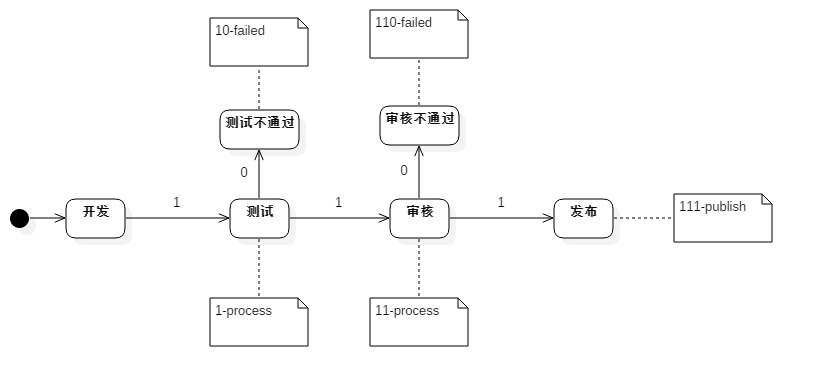
\includegraphics[width=0.8\textwidth]{image/UML/StatechartDiagram.png}
				\caption{状态图示}
				\label{fig:status}
			\end{figure}
		\end{itemize}
			
			
			
			